\documentclass[notitlepage]{math}
\usepackage{lipsum}
\usetikzlibrary{patterns,positioning, decorations, decorations.pathreplacing}
\title{Vector Spaces Chap. 11} %Titre du fichie
\author{FireGhost} %Auteur du fichier

\begin{document}
\titre{Chapter 11: Vector Spaces} %Titre du fichier .pdf
\UE{Vector Spaces} %Nom de la UE

\fairetitre
\fairemarges
% subsubsubsection
\setcounter{secnumdepth}{4}
\titleformat{\paragraph}
{\normalfont\normalsize\bfseries}{\theparagraph}{1em}{}
\titlespacing*{\paragraph}
{0pt}{3.25ex plus 1ex minus .2ex}{1.5ex plus .2ex}

\newcommand{\minus}{\scalebox{0.75}[1.0]{$-$}} % Minus sign

During this chapter, $\mathbb{K}$ will be either $\mathbb{R}$ or $\mathbb{C}$.
\section{General approach}
\subsection{Structure of a Vector Space}
Let $E$ be a set, we define two operations:\\
\newline
\begin{minipage}{0.5\linewidth}
    \begin{itemize}
    \item An internal operation: \\
    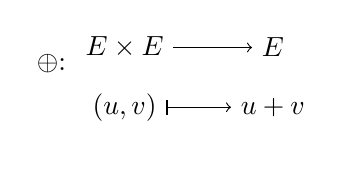
\begin{tikzpicture}[node distance=1mm]
        \node (center) at (0,0) {};
        \node (functionName) at (0, 1) {$\oplus$:};
        \node[above right = -0.3cm and 0cm of functionName] (domain) {$E \times E$};
        \node[right = 1cm of domain] (codomain) {$E$};
        \node[below = 2mm of domain] (element) {$(u , v)$};
        \node at (element-|codomain) (image) {$u+v$};
        \draw[->] (domain) -- (codomain);
        \draw[|->] (element) -- (image);
    \end{tikzpicture}
\end{itemize}
\end{minipage}
\begin{minipage}{0.5\linewidth}
    \begin{itemize}
    \item An external operation: \\
    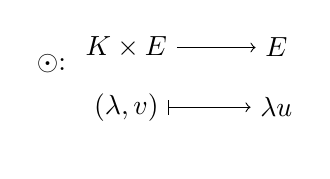
\begin{tikzpicture}[node distance=1mm]
        \node (center) at (0,0) {};
        \node (functionName) at (0, 1) {$\odot$:};
        \node[above right = -0.3cm and 0cm of functionName] (domain) {$\mathbb{K} \times E$};
        \node[right = 1cm of domain] (codomain) {$E$};
        \node[below = 2mm of domain] (element) {$(\lambda , v)$};
        \node at (element-|codomain) (image) {$\lambda u$};
        \draw[->] (domain) -- (codomain);
        \draw[|->] (element) -- (image);
    \end{tikzpicture}
\end{itemize}
\end{minipage}
\subsection{Defintion}
\noindent We say that $(E, \oplus, \odot)$ is a vector space if $\forall (u,v,w) \in E^3$ we have:
\begin{itemize}
    \item u + (v + w) = (u + v) + w {\color{green}($\oplus$ is associative)}
    \item u + v = v + u {\color{green}($\oplus$ is commutative)}
    \item $\exists 0_E \in E$ such that $u + 0_E = 0_E + u = u$ {\color{green}(Existence of a neutral element for $\oplus$)}
    \item $\exists \minus u \in E$, $u + (\minus u) = (\minus u) + u = 0_E$ {\color{green}(Existence of a symmetrical element for $\oplus$)}
\end{itemize}
And $\forall (u, v) \in E^2$ and $\forall (\alpha, \beta) \in \mathbb{K}^2$ we have:
\begin{itemize}
    \item $(\alpha + \beta) \cdot u = \alpha \cdot u + \beta \cdot u$ {\color{green}($\odot$ is distributive)}
    \item $\alpha (u + v) = \alpha \cdot u + \alpha \cdot v$ {\color{green}($\odot$ is distributive)}
    \item $(\alpha \beta) u = \alpha (\beta u)$ {\color{green}($\odot$ is associative)}
    \item $1_{\mathbb{K}} \cdot u = u$ {\color{green}(Where $1_{\mathbb{K}}$ is the neutral element of multiplication of element of $\mathbb{K}$)}
\end{itemize}
Let (E, $\oplus$, $\odot$) be a $\mathbb{K}$-Vector Space,\\
Any element from E is called a vector and any element from $\mathbb{K}$ is called a scalar.\\
$0_E$ is called the zero vector.\\
\subsubsection{Property}
$\forall u \in E$ and $\forall \alpha \in \mathbb{K}$ we have:
\begin{enumerate}
    \item $\alpha \cdot 0_E = 0_E$
    \item $0_{\color{red}\mathbb{K}} \cdot u = 0_{\color{red}E}$
    \item $\alpha \cdot u = 0_E \Leftrightarrow \alpha = 0_{\color{red}\mathbb{K}}$ or $u = 0_{\color{red}E}$
\end{enumerate}
\subsubsection{Example}
\begin{enumerate}
    \item $E = \mathbb{R}^2$, $U = \begin{pmatrix} 1 \\ 1 \end{pmatrix} \in \mathbb{R}^2$
    \item $\mathbb{R}^3 , \mathbb{R}^4, \dots , \mathbb{R}^n$ are $\mathbb{R}-VS$
    \item $\mathbb{R}[X]:$ Set of polynomials \\
    $0_{\mathbb{R}[X]}: \mathbb{R}_2[X] = \left\{aX^2 + bX + c , (a,b,c) \in \mathbb{R}^3\right\}$\\
    $\mathbb{R}_2$ means: "at least max2", here "a" can be 0
    \item $\mathbb{R}^\mathbb{N}$ and $\mathbb{R}^\mathbb{R}$ are $\mathbb{R}$-VS \\ \\
    ex: $\left.\left(\frac{1}{n}\right)_{n\in\mathbb{N}^\ast}\right\}$ VS: 8 Property are check
\end{enumerate}
\subsection{Vector Subspaces (= linear subspaces)}
\subsubsection{Definition}
Let $E$ be a $\mathbb{K}$-Vector Space:\\
\begin{itemize}
    \item $F \subset E$ {\color{green}(F is a subset of E)}
    \item $F \neq \emptyset$ {\color{green}(F is non-empty, $0_E \in F$)}
    \item $\forall (u, v) \in F^2$, $\forall \alpha \in \mathbb{K}$, $(\alpha \cdot u + v) \in F$ {\color{green}(F is closed under linear combination)}
\end{itemize}
\subsubsection{Propositions}
\paragraph{Proposition 1}
Let $E$ be a $\mathbb{K}$-Vector Space:
\begin{align*}
    F \subset E \text{ is a Vector SubSpace of } E &\Longrightarrow 0_E \in F\\
    &\;\not\!\!\!\Longleftarrow  
\end{align*}
\paragraph{Example}
\noindent $E = \mathbb{R}^3$\\
$F_1 = \left\{\begin{pmatrix} x\\ y\\ z \end{pmatrix} \in \mathbb{R}^3, x + y + z = 1\right\}$ and $F'_1 = \left\{\begin{pmatrix} x\\ y\\ z \end{pmatrix} \in \mathbb{R}^3, x + y + z = 0\right\}$\\
$0_E \notin F_1 \Longrightarrow F_1$ is not a Vector SubSpace of $E$\\
$\forall (u, v) \in {F'}_1^2$, $\forall \alpha \in \mathbb{R}$, $u = \begin{pmatrix} x\\ y\\ z \end{pmatrix}$ and $v = \begin{pmatrix} x'\\ y'\\ z' \end{pmatrix}$\\
$\alpha u + v = \alpha(x, y, z) + (x', y', z') = 0_E \in F'_1$
$\Longrightarrow F'_1$ is a Vector SubSpace of $E$\\
\\
\noindent
$F_2 = \left\{\begin{pmatrix} x\\ y \end{pmatrix} \in \mathbb{R}^2 {\color{green} \begin{cases} \in \mathbb{R}^3 \\ \ni 0_E \end{cases}},{\color{green}0_E \in } x y \ge 0\right\}$ \\
$\left( \begin{pmatrix}
    1 \\ 0 \end{pmatrix} , \begin{pmatrix}
    0 \\ -1 \end{pmatrix}\right) \in {F_2}^2$ \\
$\begin{pmatrix}
1 \\ 0 \end{pmatrix} + \begin{pmatrix}
0 \\ -1 \end{pmatrix} = \begin{pmatrix} 1 \\ -1 \end{pmatrix} \notin {F_2}^2$ Not closed by linear combination \\
\\
Exercise on your own: 
$F_3 = \left\{P \in \mathbb{R}[X], P(2) = 0 \right\}$



\paragraph{Proposition 2}
Let $E$ be a Vector Space, $F$ and $G$ two Vector SubSpaces of $E$. Then:\\
\begin{enumerate}
    \item $F \cap G \subset E$,    $F \cap G$ is a Vector SubSpace of $E$
    \item $\left.\begin{matrix}
        F \text{ VSS of }E \implies 0_E \in F \\
        G \text{ VSS of }E \implies 0_E \in G
    \end{matrix} \text{ } \right| \implies 0_E \in F \cap G \implies F \cap G \ne \emptyset$
    \item $\forall (u,v) \in F\cap G, \forall \alpha \in \mathbb{K}$ Then: $F$ close under linear combination
    \\ 
    $\left. \begin{matrix} \implies \alpha u + v \in F. \\ \text{So far for G }\implies \alpha u + v \in G  \end{matrix} \right\} \alpha u + v \in F\cap G $ \\ and $F\cap G$ is closed under linear combination.
\end{enumerate} 
\paragraph{Proposition 3}
Let $E$ be a VS: $\{0_E\}$ (sigleton) is a VSS of $E$
\paragraph{Proof:}
\begin{enumerate}
    \item $\{0_E\} \subset E$
    \item $0_E \in \{0_E\} \implies \{0_E\} \ne \emptyset $
    \item $ \forall (u,v) \in {\{0_E\}}^2, u = v = 0_E$ and $\forall \alpha \in \mathbb{K}, \alpha u = 0_E \implies \alpha u + v = 0_E \implies (\alpha u + v) \in \{0_E\}$
\end{enumerate}
\paragraph{Proposition 4}
Let $(E, \oplus , \odot)$ be a VS and $F$ a VSS of $E$, then $F$ is a VS
\subsection{Sum  of VSS}
Let $E$ a $\mathbb{K}$-VS, $F$ and $G$ VSS of $E$, we say $H$ is the sum of $F$ and $G$ if:

\[H = \left\{u \in E, \exists (v,w)  \in F \times G, u = v + w \right\}\]
\subsection{Examples}
\begin{enumerate}
    \item $ E = \mathbb{R}^2, G = \left\{ \begin{pmatrix}
        x \\ 0 \end{pmatrix}, x \in \mathbb{R} \right\}, 
        H = \left\{ \begin{pmatrix} 0 \\ y \end{pmatrix}, y \in \mathbb{R} \right\}$ \\
        $ G + H = \left\{ \begin{pmatrix} x \\ y \end{pmatrix}, (x,y) \in \mathbb{R}^2 = \mathbb{R}^2 \right\}$
    \item $\left. \begin{matrix} 
        F = \left\{ \begin{pmatrix} x \\ 0 \\ 0 \end{pmatrix},x \in \mathbb{R}   \right\}\\
        G = \left\{ \begin{pmatrix} 0 \\ 0 \\ z \end{pmatrix},z \in \mathbb{R}   \right\}
    \end{matrix} \right\}$ VSS of $\mathbb{R}^3$ \\
    $F+G  = \left\{ \begin{pmatrix} x \\ 0 \\ z \end{pmatrix},(x,z) \in \mathbb{R}^2  \right\} \in \mathbb{R}^3 \ne \mathbb{R}^3$
\end{enumerate}
\subsection{Direct Sum}
\subsubsection{Definition}
Let $E$ a $\mathbb{K}$-VS, $F$ and $G$ two VSS of $E$,\\ we say that $F$ and $G$ are in direct sum if: 
\[F\cap G = \{0_E\}\]
\subsubsection{Notation}
In that case we denote $F \oplus G$ instead of $ F + G$
\subsubsection{Examples}
\begin{enumerate}
    \item Both of previous examples
    \item $\left. \begin{matrix} 
        F = \left\{ \begin{pmatrix} x \\ y \\ z \end{pmatrix},z = 0, x , y \in \mathbb{R}^2   \right\}\\
        G = \left\{ \begin{pmatrix} x \\ 0 \\ z \end{pmatrix}, (x,y) \in \mathbb{R}^2   \right\}
    \end{matrix} \right\}
    \begin{pmatrix}
        1 \\ 0 \\ 0 
    \end{pmatrix} \in F \cap G    $ \\
    $F+G$  Check\\
    $F \oplus G$  Not bc $F \cap G \ne \{0_E\}$

    

\end{enumerate}
\end{document}